\documentclass[tikz,border=10pt]{standalone}
\usetikzlibrary{positioning, arrows.meta}

\begin{document}
	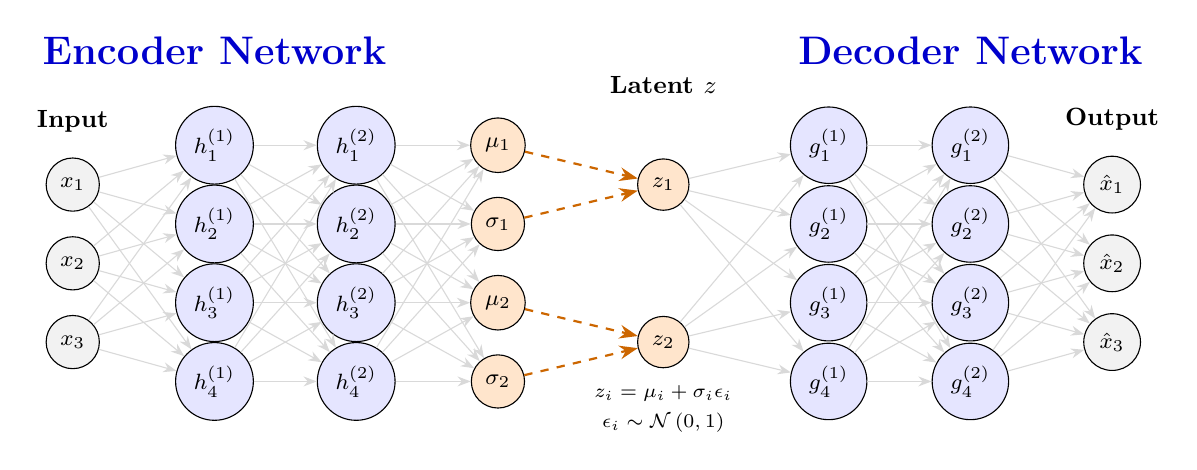
\begin{tikzpicture}[
		>=Stealth,
		node distance=1.2cm and 1.8cm,
		neuron/.style={draw, circle, minimum size=0.6cm, font=\footnotesize, fill=blue!10},
		latent/.style={draw, circle, minimum size=0.6cm, font=\footnotesize, fill=orange!20},
		io/.style={draw, circle, minimum size=0.6cm, font=\footnotesize, fill=gray!10},
		label_font/.style={font=\small\bfseries}
		]
		
		% --- ENCODER ---
		% Input Layer (3 nodes)
		\foreach \i in {1,...,3} {
			\node[io] (x\i) at (0, 1.5 - \i*1.0) {$x_\i$};
		}
		\node[above=0.2cm of x1, label_font] {Input};
		
		% Encoder Hidden 1 (4 nodes)
		\foreach \i in {1,...,4} {
			\node[neuron] (eh1_\i) at (1.8, 2.0 - \i*1.0) {$h^{(1)}_\i$};
		}
		
		% Encoder Hidden 2 (4 nodes)
		\foreach \i in {1,...,4} {
			\node[neuron] (eh2_\i) at (3.6, 2.0 - \i*1.0) {$h^{(2)}_\i$};
		}
		
		% --- LATENT SPACE (BOTTLENECK) ---
		% Parameters mu and sigma (2 nodes each)
		\node[latent] (mu1) at (5.4, 1.0) {$\mu_1$};
		\node[latent] (mu2) at (5.4, 0.0) {$\sigma_1$};
		\node[latent] (sig1) at (5.4, -1.0) {$\mu_2$};
		\node[latent] (sig2) at (5.4, -2.0) {$\sigma_2$};
		
		% Latent vector z (2 nodes)
		\node[latent] (z1) at (7.5, 0.5) {$z_1$};
		\node[latent] (z2) at (7.5, -1.5) {$z_2$};
		\node[above=0.7cm of z1, label_font] {Latent $z$};
		
		% --- DECODER ---
		% Decoder Hidden 1 (4 nodes)
		\foreach \i in {1,...,4} {
			\node[neuron] (dh1_\i) at (9.6, 2.0 - \i*1.0) {$g^{(1)}_\i$};
		}
		
		% Decoder Hidden 2 (4 nodes)
		\foreach \i in {1,...,4} {
			\node[neuron] (dh2_\i) at (11.4, 2.0 - \i*1.0) {$g^{(2)}_\i$};
		}
		
		% Output Layer (3 nodes)
		\foreach \i in {1,...,3} {
			\node[io] (xhat\i) at (13.2, 1.5 - \i*1.0) {$\hat{x}_\i$};
		}
		\node[above=0.2cm of xhat1, label_font] {Output};
		
		
		% --- FULLY CONNECTED EDGES ---
		% Input -> Enc H1
		\foreach \i in {1,...,3} {
			\foreach \j in {1,...,4} {
				\draw[->, draw=black!15] (x\i) -- (eh1_\j);
			}
		}
		
		% Enc H1 -> Enc H2
		\foreach \i in {1,...,4} {
			\foreach \j in {1,...,4} {
				\draw[->, draw=black!15] (eh1_\i) -- (eh2_\j);
			}
		}
		
		% Enc H2 -> Mu & Sigma
		\foreach \i in {1,...,4} {
			\draw[->, draw=black!15] (eh2_\i) -- (mu1);
			\draw[->, draw=black!15] (eh2_\i) -- (mu2);
			\draw[->, draw=black!15] (eh2_\i) -- (sig1);
			\draw[->, draw=black!15] (eh2_\i) -- (sig2);
		}
		
		% Reparameterization Sampling (Mu & Sigma -> z)
		\draw[->, thick, dashed, draw=orange!80!black] (mu1) -- (z1);
		\draw[->, thick, dashed, draw=orange!80!black] (mu2) -- (z1);
		\draw[->, thick, dashed, draw=orange!80!black] (sig1) -- (z2);
		\draw[->, thick, dashed, draw=orange!80!black] (sig2) -- (z2);
		
		% Sampling Equation Label
		\node[below=0.1cm of z2, font=\scriptsize\itshape, align=center] {$z_i = \mu_i + \sigma_i \epsilon_i$ \\[0.1cm] $\epsilon_i \sim \mathcal{N} \left(0, 1 \right) $};
		
		% z -> Dec H1
		\foreach \i in {1,2} {
			\foreach \j in {1,...,4} {
				\draw[->, draw=black!15] (z\i) -- (dh1_\j);
			}
		}
		
		% Dec H1 -> Dec H2
		\foreach \i in {1,...,4} {
			\foreach \j in {1,...,4} {
				\draw[->, draw=black!15] (dh1_\i) -- (dh2_\j);
			}
		}
		
		% Dec H2 -> Output
		\foreach \i in {1,...,4} {
			\foreach \j in {1,...,3} {
				\draw[->, draw=black!15] (dh2_\i) -- (xhat\j);
			}
		}
		
		% --- TOP NETWORK TITLE LABELS ---
		\node[font=\Large\bfseries, color=blue!80!black] at (1.8, 2.2) {Encoder Network};
		\node[font=\Large\bfseries, color=blue!80!black] at (11.4, 2.2) {Decoder Network};
		
	\end{tikzpicture}
\end{document}
